\documentclass[11pt,a4paper,dvipdfmx]{jlreq}

% 必須パッケージ
\usepackage[dvipdfmx]{graphicx} % 画像読み込み
\usepackage{caption}            % minipage内でキャプションをつけるため
\usepackage{amsmath,amssymb}
\usepackage{url}

% ページ余白の調整（図を大きく見せるため少し余白を狭くする設定）
\usepackage[top=25mm, bottom=25mm, left=20mm, right=20mm]{geometry}

% タイトル情報
\title{CO$_2$貯留・放散装置向け制御基板(M304)用\\パラメータ変換書き込みシステム 仕様書}
\author{ラボサポート九州　－Lab Support Q-shu－}
\date{\today}

\begin{document}

\maketitle

\begin{abstract}
本ドキュメントは，Webアプリケーションから入力された制御パラメータをM304デバイスのEEPROMに書き込むための，
システム全体の動作仕様および各スクリプトの処理フローについてまとめたものである．
各モジュールのデータフローと変換プロセスを可視化し，システム全体の挙動を定義する．
\end{abstract}

\tableofcontents
\clearpage

% ==========================================
\section{システムの全体シーケンス}

\noindent
% 左側のブロック（幅を全体の55%に設定）
\begin{minipage}[t]{0.55\textwidth}
    \vspace{0pt} 
    \centering
    % 高さをテキスト領域の85%に制限してページオーバーを防ぐ
    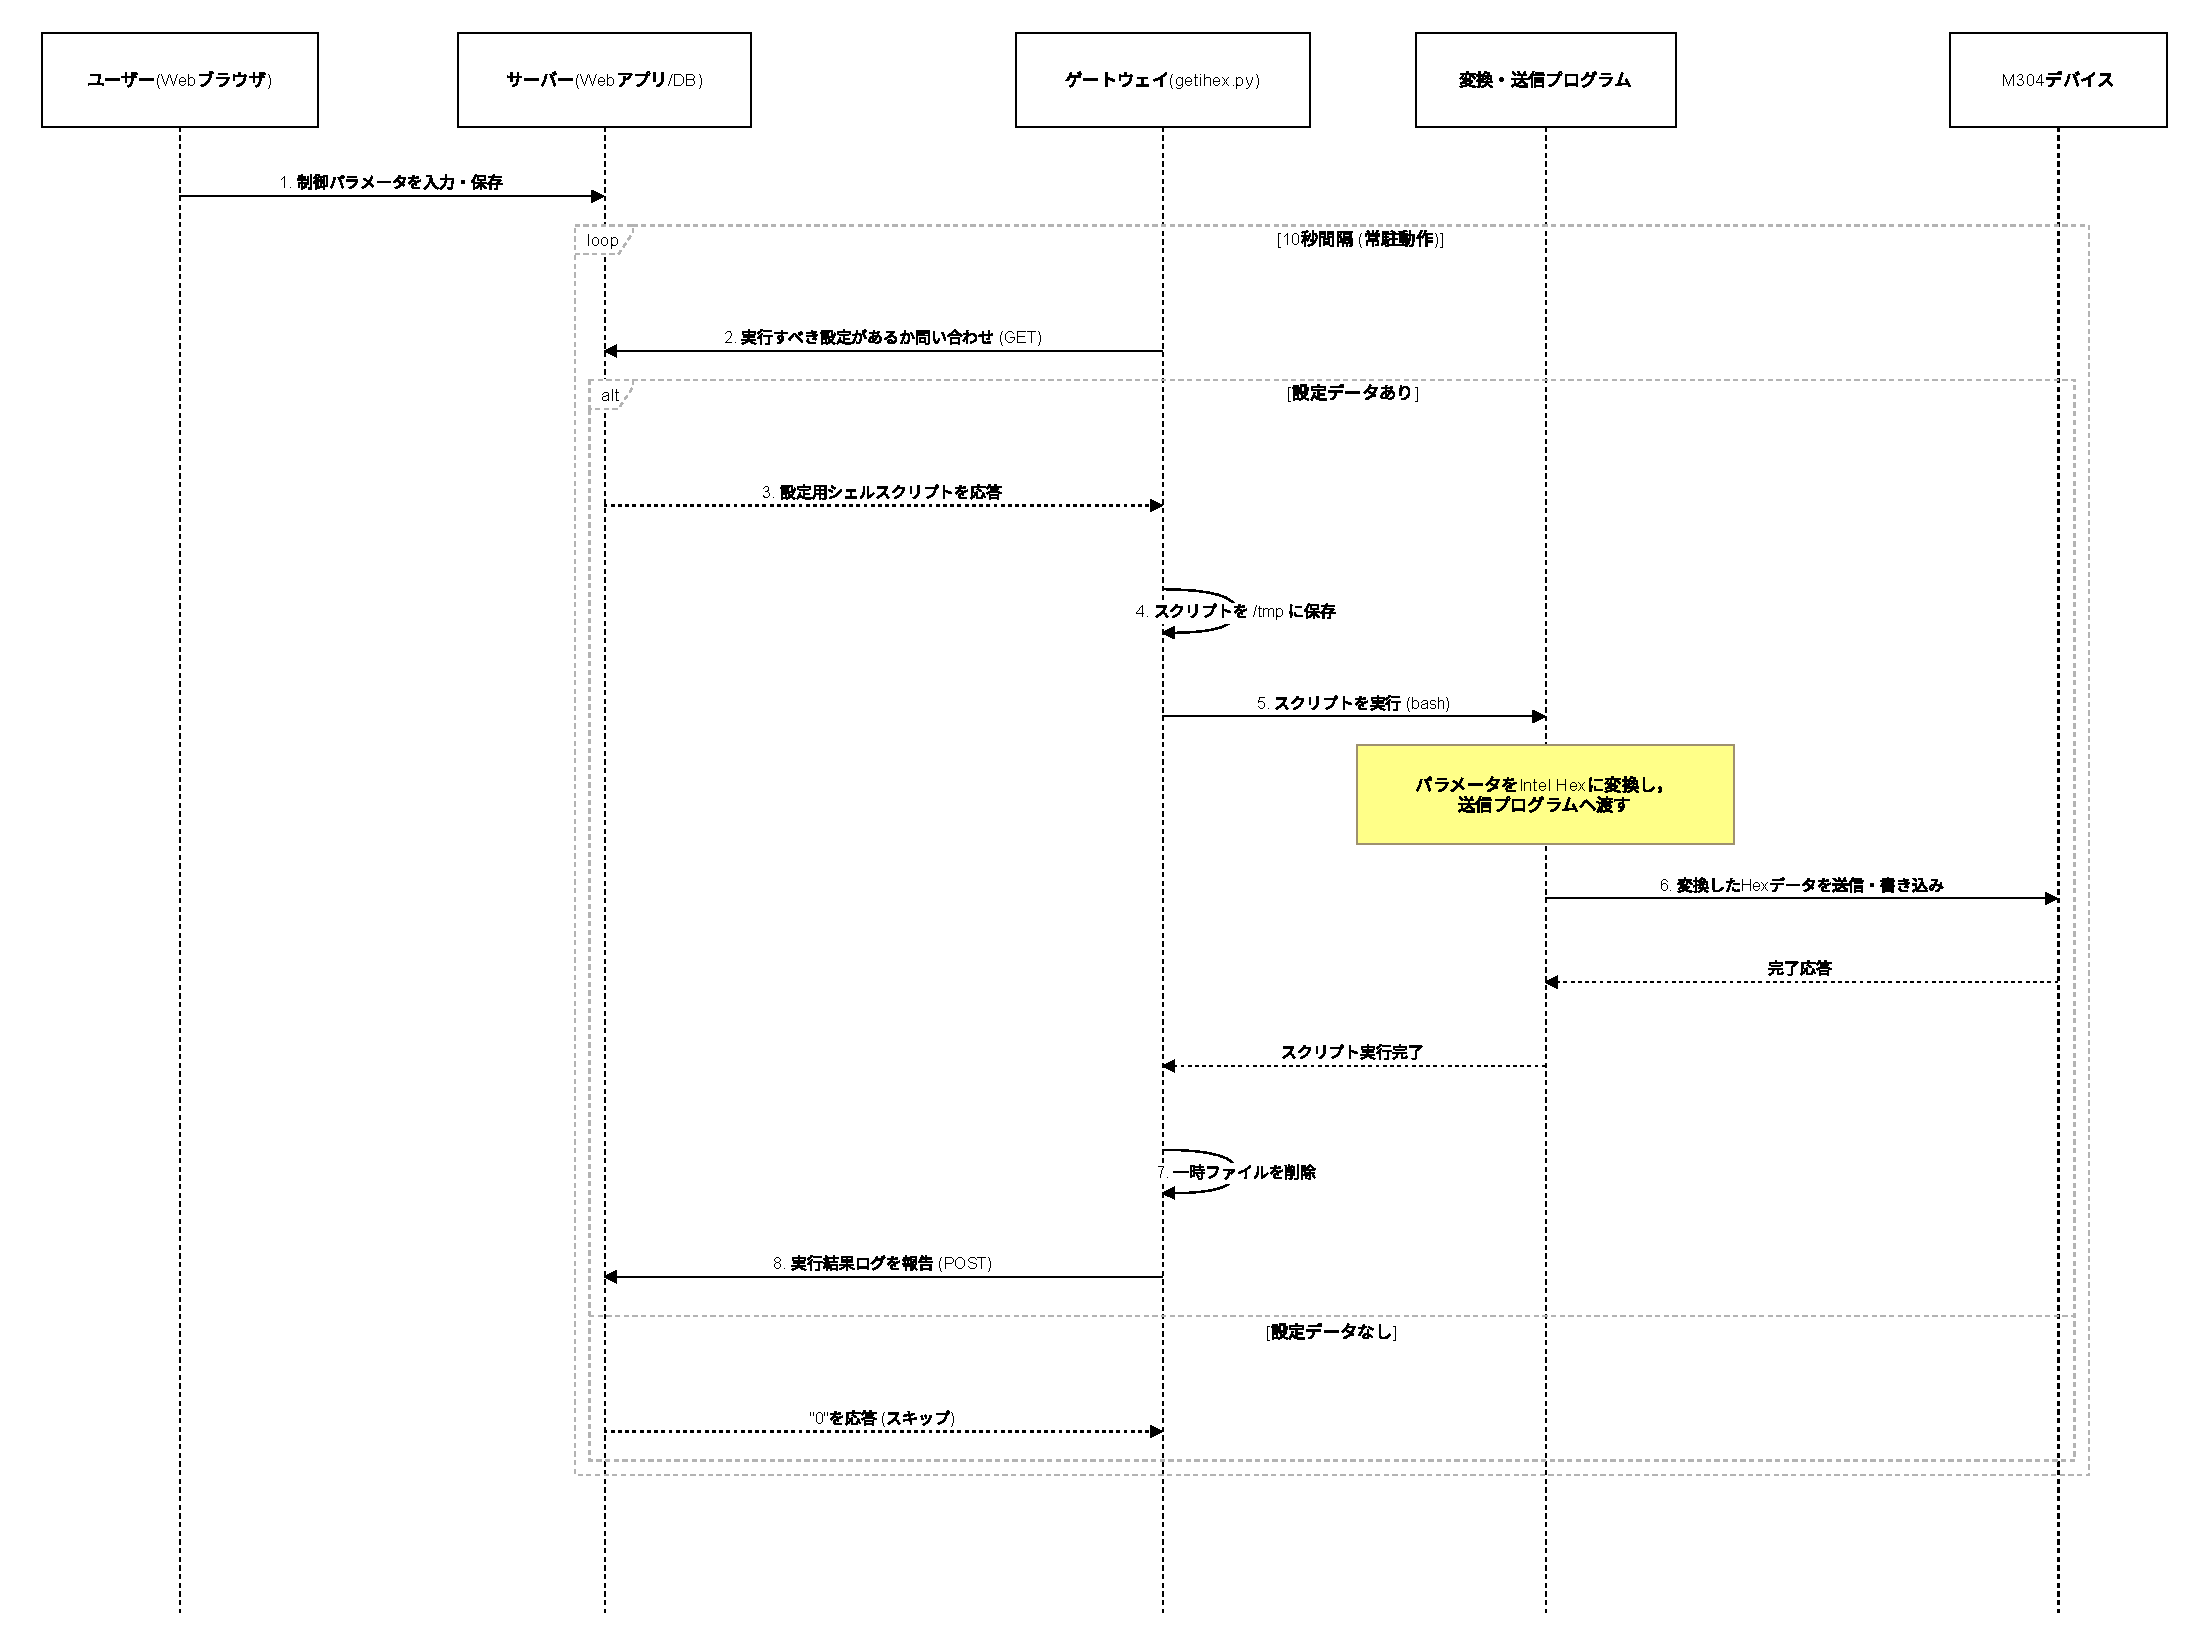
\includegraphics[width=\linewidth, height=0.85\textheight, keepaspectratio]{mkihex.drawio.pdf}
    \captionof{figure}{システム全体シーケンス}
    \label{fig:sequence}
\end{minipage}
\hfill
% 右側のブロック（幅を全体の40%に設定）
\begin{minipage}[t]{0.4\textwidth}
    \vspace{0pt}
    ユーザーがWebブラウザからパラメータを入力し，
    M304デバイスにデータが書き込まれるまでの全体的な処理の流れを左図に示す．
    
    ゲートウェイ上で常駐する \texttt{getihex.py} が10秒間隔でサーバーへ問い合わせ(GETリクエスト)を行い，
    実行すべき設定データが存在する場合に，設定用シェルスクリプトを一時ファイルとしてダウンロードして実行する．
    
    スクリプトの実行によってパラメータがIntel Hex形式に変換・送信され，デバイスへの書き込みが完了すると，
    一時ファイルは削除され，実行結果のログがサーバーへ報告(POSTリクエスト)されるプル型(Pull型)のアーキテクチャとなっている．
\end{minipage}

\clearpage

% ==========================================
\section{パラメータ変換と送信のデータフロー}

\noindent
\begin{minipage}[t]{0.55\textwidth}
    \vspace{0pt}
    \centering
    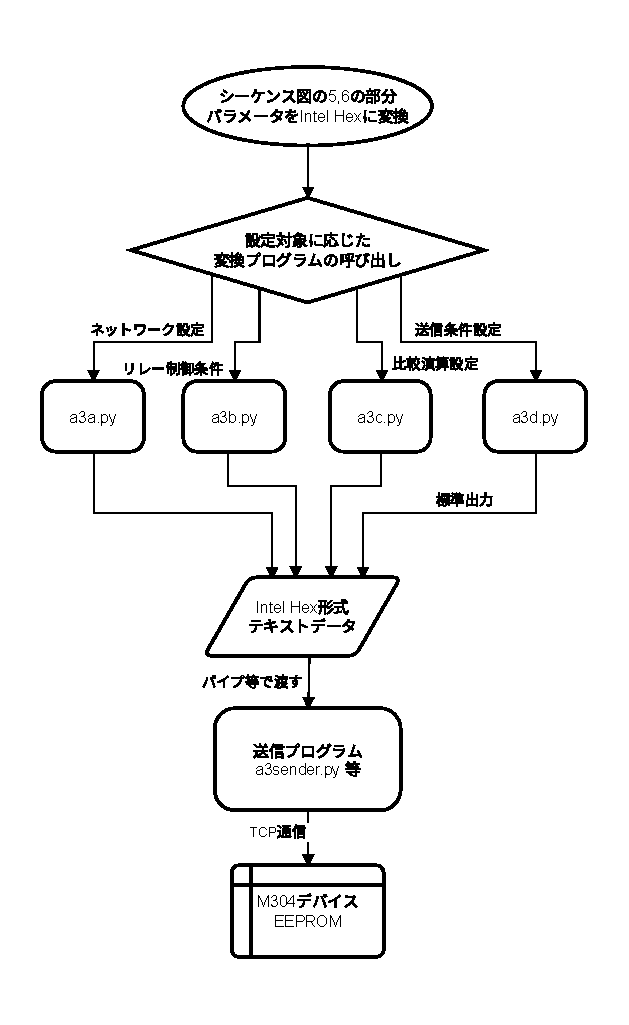
\includegraphics[width=\linewidth, height=0.85\textheight, keepaspectratio]{flowchart-mkihex.drawio.pdf}
    \captionof{figure}{パラメータからIntel Hex形式への変換と送信フロー}
    \label{fig:flowchart-mkihex}
\end{minipage}
\hfill
\begin{minipage}[t]{0.4\textwidth}
    \vspace{0pt}
    ダウンロードされた設定用シェルスクリプトが実行された際の，設定対象に応じたデータ変換のパイプラインを左図に示す．
    
    処理は以下の手順で構成される：
    \begin{itemize}
        \item \textbf{変換スクリプトの呼び出し}:\\
        設定項目（ネットワーク設定，リレー制御条件，比較演算設定，送信条件設定）に応じて，
        適切なPythonスクリプト(\texttt{a3a.py} $\sim$ \texttt{a3d.py})が呼び出される．
        \item \textbf{Hexデータの受け渡し}:\\
        各スクリプトの標準出力から生成されたIntel Hex形式のテキストデータは，
        パイプ($|$)等を経由して送信プログラムに渡される．
        \item \textbf{デバイスへの送信}:\\
        送信プログラム（\texttt{a3sender.py} 等）が，
        受け取ったHexデータをTCP/シリアル通信などを介してM304デバイスのEEPROMの所定のアドレス帯域へ書き込む．
    \end{itemize}
\end{minipage}

\clearpage

% ==========================================
\section{インテルヘキサ変換プログラム (\texttt{a3X.py})}

\noindent
\begin{minipage}[t]{0.55\textwidth}
    \vspace{0pt}
    \centering
    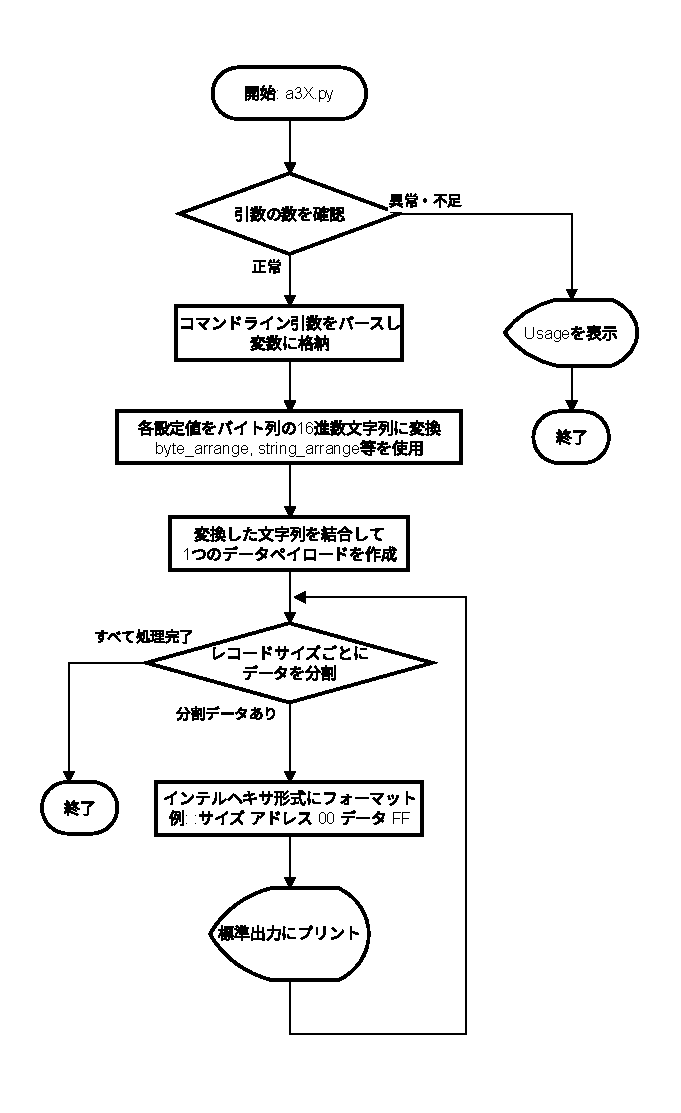
\includegraphics[width=\linewidth, height=0.85\textheight, keepaspectratio]{a3X.drawio.pdf}
    \captionof{figure}{\texttt{a3X.py} (Hexデータ生成) のフローチャート}
    \label{fig:a3X}
\end{minipage}
\hfill
\begin{minipage}[t]{0.4\textwidth}
    \vspace{0pt}
    各種パラメータを，M304が解釈可能なIntel Hex形式に変換するスクリプト群
    (\texttt{a3a.py}, \texttt{a3b.py}, \texttt{a3c.py}, \texttt{a3d.py})の共通の処理フローを左図に示す．
    
    実行時に渡されたコマンドライン引数の数を検証し，不足や異常がある場合はUsageを表示して終了する．
    正常な場合は引数をパースし，\texttt{byte\_arrange} や \texttt{string\_arrange} などの内部関数を用いて，
    IPアドレスや文字列，リレーの動作条件などの設定値をバイト列の16進数文字列に変換する．
    
    その後，変換した文字列を結合して1つのデータペイロードを作成し，規定のレコードサイズごとに分割して
    「\texttt{:サイズ アドレス 00 データ FF}」というIntel Hex形式にフォーマットし，標準出力へプリントする．
\end{minipage}

\clearpage

% ==========================================
\section{送信・ダンプ表示プログラム (\texttt{a3sender.py})}

\noindent
\begin{minipage}[t]{0.55\textwidth}
    \vspace{0pt}
    \centering
    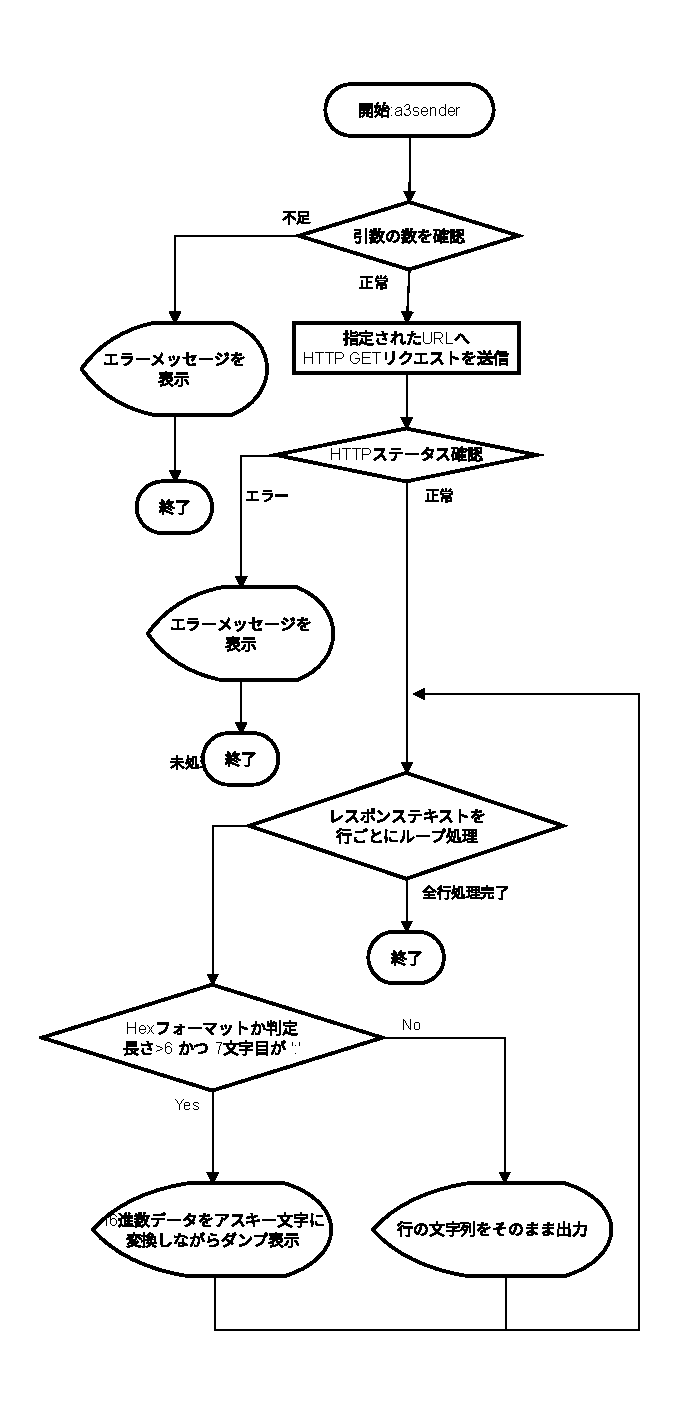
\includegraphics[width=\linewidth, height=0.85\textheight, keepaspectratio]{a3sender.drawio.pdf}
    \captionof{figure}{\texttt{a3sender.py}のフローチャート}
    \label{fig:a3sender}
\end{minipage}
\hfill
\begin{minipage}[t]{0.4\textwidth}
    \vspace{0pt}
    生成されたデータを受け取り，ダンプ表示や送信処理の基盤となるプログラムのフローを左図に示す．
    
    引数として指定されたURLへHTTP GETリクエストを送信し，レスポンステキストを取得する．
    HTTPステータスがエラーの場合は適切にエラーメッセージを表示して終了する．
    
    正常にデータを取得できた場合，レスポンスを行ごとにループ処理する．
    行の長さが6文字以上かつ7文字目が「\texttt{:}」である場合をHexフォーマットと判定し，
    該当する16進数データをアスキー文字に変換しながら人間が読める形式でダンプ表示する．
    Hexフォーマットに該当しない行はそのまま出力される．
\end{minipage}

\end{document}